%%%%%%%%%%%%%%%%%%%%%%%%%%%%%%%%%%%%%%%%%
% University Assignment Title Page
% LaTeX Template
% Version 1.0 (27/12/12)
%
% This template has been downloaded from:
% http://www.LaTeXTemplates.com
%
% Original author:
% WikiBooks (http://en.wikibooks.org/wiki/LaTeX/Title_Creation)
%
% License:
% CC BY-NC-SA 3.0 (http://creativecommons.org/licenses/by-nc-sa/3.0/)
%
% Instructions for using this template:
% This title page is capable of being compiled as is. This is not useful for
% including it in another document. To do this, you have two options:
%
% 1) Copy/paste everything between \begin{document} and \end{document}
% starting at \begin{titlepage} and paste this into another LaTeX file where you
% want your title page.
% OR
% 2) Remove everything outside the \begin{titlepage} and \end{titlepage} and
% move this file to the same directory as the LaTeX file you wish to add it to.
% Then add \input{./title_page_1.tex} to your LaTeX file where you want your
% title page.
%
%%%%%%%%%%%%%%%%%%%%%%%%%%%%%%%%%%%%%%%%%
%\title{Title page with logo}
%----------------------------------------------------------------------------------------
%	PACKAGES AND OTHER DOCUMENT CONFIGURATIONS
%----------------------------------------------------------------------------------------

\documentclass[12pt]{article}
\usepackage[english]{babel}
\usepackage[utf8x]{inputenc}
\usepackage{amsmath}
\usepackage{graphicx}
\usepackage[colorinlistoftodos]{todonotes}

%\usepackage{setspace}
%\doublespacing

\begin{document}

	\begin{titlepage}

		\newcommand{\HRule}{\rule{\linewidth}{0.5mm}} % Defines a new command for the horizontal lines, change thickness here

		\center % Center everything on the page

		%----------------------------------------------------------------------------------------
		%	HEADING SECTIONS
		%----------------------------------------------------------------------------------------

		\textsc{\LARGE Simon Fraser University}\\[1.5cm] % Name of your university/college
		\textsc{\Large Project report for MBB 496}\\[0.5cm] % Major heading such as course name
		\textsc{\large Honours Project}\\[0.5cm] % Minor heading such as course title

		%----------------------------------------------------------------------------------------
		%	TITLE SECTION
		%----------------------------------------------------------------------------------------

		\HRule \\[0.4cm]
		{ \bfseries IslandCompare: Enabling Phyletic-Based Comparison and Visualization of Genomic Islands for Tens to Hundreds of Microbial Genomes}\\[0.4cm] % Title of your document
		\HRule \\[1.5cm]

		%----------------------------------------------------------------------------------------
		%	AUTHOR SECTION
		%----------------------------------------------------------------------------------------

		\begin{minipage}{0.4\textwidth}
			\begin{flushleft} \large
				\emph{Authors:}\\
				Adrian \textsc{Lim} \\
			\end{flushleft}
		\end{minipage}
		~
		\begin{minipage}{0.4\textwidth}
			\begin{flushright} \large
				\emph{Supervisors:} \\
				Dr. Fiona \textsc{Brinkman} % Supervisor's Name

				Dr. Claire \textsc{Bertelli} % Supervisor's Name
			\end{flushright}
		\end{minipage}\\[2cm]

		% If you don't want a supervisor, uncomment the two lines below and remove the section above
		%\Large \emph{Author:}\\
		%John \textsc{Smith}\\[3cm] % Your name

		%----------------------------------------------------------------------------------------
		%	DATE SECTION
		%----------------------------------------------------------------------------------------

		{\large \today}\\[2cm] % Date, change the \today to a set date if you want to be precise

		%----------------------------------------------------------------------------------------
		%	LOGO SECTION
		%----------------------------------------------------------------------------------------

		
\includegraphics{SFUlogo.png}\\[1cm] % Include a department/university logo - this will require the graphicx package

		%----------------------------------------------------------------------------------------

		\vfill % Fill the rest of the page with whitespace

	\end{titlepage}

	\begin{abstract}
		Genomic islands, clusters of genes acquired by horizontal transfer, are frequently associated with medically important features such as virulence and anti-microbial resistance genes.\cite{3_dobrindt_2004, 4_hackerkaper_2000} Web accessible tools such as IslandViewer facilitate the creation of interactive visualizations used to study genomic islands.\cite{2_islandviewer3} These tools, however, only allow the viewing of 1 or 2 genomes at a time. This becomes cumbersome when attempting to compare multiple genomes particularly in genetic epidemiology where many genomes need to be compared and analyzed rapidly. IslandCompare is an interactive web-based application that has been designed to enable the rapid prediction and visualization of genomic islands and other genomic features across tens to hundreds of microbial genomes. 
	\end{abstract}

	\section{Introduction}
        
	\section{Implementation}
	
	\subsection{Web Interface}
		IslandCompare was built with the Django web framework.\cite{8_django_2016} Users will be able to upload their own genomes and select subsets of them to run through the IslandCompare pipeline. From the web interface, users can also see the status and results of their analyses.
	
	\subsection{Data Processing Pipeline}
		An IslandCompare job consists of multiple tasks in order to create a visualization. These tasks consist of phylogenetic tree construction, multiple sequence alignment, genomic island prediction and clustering. Many of these tasks are dependent on others and are therefore run sequentially. Some of these tasks however are independent and can run in parallel with other tasks. Though having multiple different tasks run in parallel increases complexity of the system, it allows better utilization of resources in a multi threaded or distributed environment. Celery, a distributed task queue, is used to manage processing of data in this system.\cite{9_celery} A flowchart of the IslandCompare pipeline can be seen in figure \ref{fig:islandcomparepipeline}.
		
		\begin{figure}[h]
			\centering
			\includegraphics[width=0.6\textwidth]{IslandComparePipelineV2}
			\caption{\label{fig:islandcomparepipeline} Flowchart of Data through IslandCompare}
		\end{figure}
	
	\subsubsection{Phylogenetic Tree Construction}
		Although IslandCompare will use a user's phylogenetic tree if it is provided, it is capable of generating its own if none is provided. It generates phylogenetic trees by using Parsnp.\cite{7_treangen_ondov_koren_phillippy_2014}
	
	\subsubsection{Multiple Sequence Alignment}
		IslandCompare generates a multiple sequence alignment using Mauve.\cite{10_mauve} In IslandCompare, Mauve is run for each adjacent pair of sequences in the phylogenetic tree. This has many benefits including avoiding limitations we ran into concerning the maximum number of sequences Mauve can run in a single execution. In constructing our alignment in this way we eliminate the comparisons against sequences not adjacent to each other in the phylogenetic tree and thereby improve the performance and memory usage of this program in IslandCompare.
	
	\subsubsection{Genomic Island Prediction}
		Genomic islands are predicted using Sigi-HMM.\cite{11_sigihmm}
		
	\subsubsection{Clustering of Genomic Islands}
		Genomic islands are clustered by using Mash and Markov Clustering.\cite{12_mash, 13_mcl}
	
	\subsubsection{Genomic Island Visualization}	
		The visualization component of IslandCompare was developed using the D3 JavaScript library.\cite{6_d3}
		
		\begin{figure}[h]
			\centering
			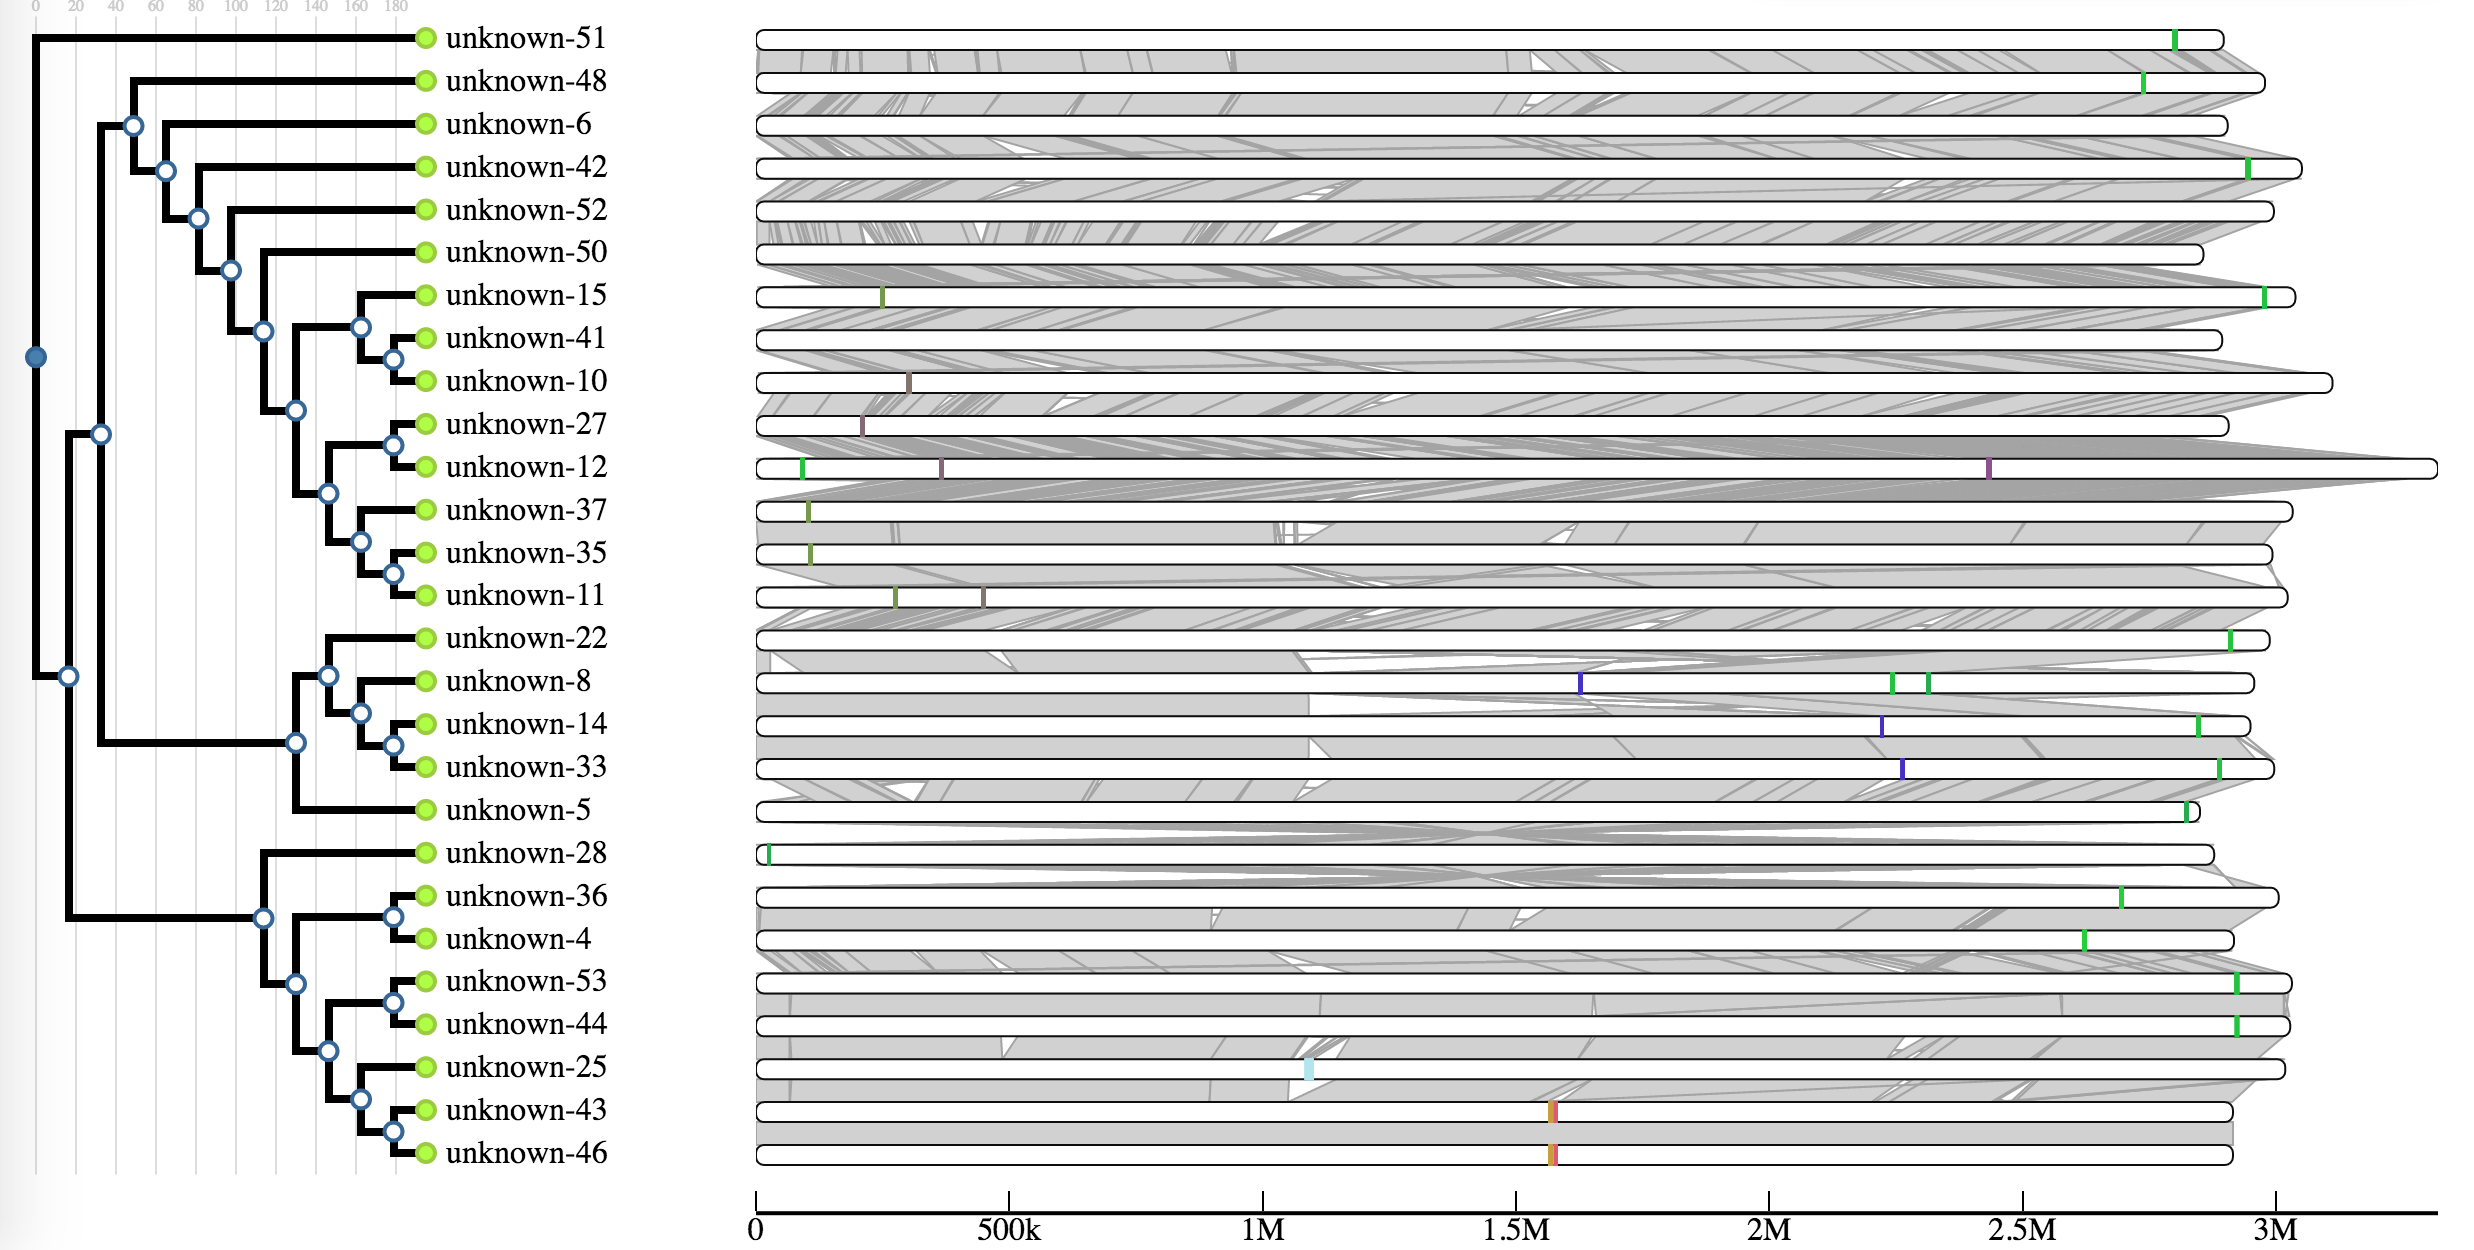
\includegraphics[width=0.8\textwidth]{IslandCompare}
			\caption{\label{fig:islandcompare} Visualization Generated by IslandCompare of 50 Sequences}
		\end{figure}

	\section{Concluding Comments}

	\clearpage
	\bibliography{report}
	\bibliographystyle{ieeetr}

\end{document}